\chapter{Method of Approach}
\label{ch:method}

This chapter will focus on the implementation of the software tool initially proposed in Chapter \ref{ch:intro}. The overall software is composed of three separate tools, an installer, an interface, and a Dockerfile generator. The primary language used for this project is Python due to packages available within Python and the ease to add and import external packages. Two main packages are being utilized for the creation of the tool which is the Docker Python \cite{dockerPython} wrapper for interacting with Docker and Flask \cite{flask} for building the browser-based interface.

\break

% This chapter should answer the ``how'' question - how did you complete your project, including the overall design of your study, details of the algorithms and tools you have used, etc.
%  Use technical diagrams, equations, algorithms, and paragraphs of text to
% describe the research that you have completed. Be sure to number all figures and tables and to explicitly refer to them in your text.

The software tool, that I have developed, as previously mentioned has three main components. The Docker Installer, the Interface, and the Dockerfile Generator. Each of these components works together to ensure optimum user experience. The installer ensures that the user will be able to properly use Docker, the Interface, and the Dockerfile Generator. The Interface allows the user to easily use the Dockerfile Generator and interact with the more common Docker commands. The Dockerfile Generator allows the user to easily create Docker images that the Interface can run. The overall file structure of the tool can be seen in Figure \ref{fig:fileStruct} below.

\begin{figure}[h!]
  \dirtree{%
.1 Docker-Automation/.
.2 auto/\DTcomment{Main Utilities and Program Files}.
.3 containers\DTcomment{Container Utilities Program File}.
.3 docker\_auto\DTcomment{Command Line Interface Program File}.
.3 generate\DTcomment{Dockerfile Generator Program File}.
.3 images\DTcomment{Image Utilities Program File}.
.3 install\DTcomment{Installation Functions Program File}.
.2 interface/\DTcomment{Flask Interface and Style Files}.
.3 static/\DTcomment{Static Files Used for Interface Construction}.
.3 templates/\DTcomment{HTML Pages for Interface}.
.3 interface\_containers\DTcomment{Containers Interface Utilities Page}.
.3 interface\_main\DTcomment{Main Interface Page}.
.3 interface\_images\DTcomment{Images Interface Utilities Page}.
.2 tests/\DTcomment{Tests to Ensure Utilities Function Properly}.
.2 samples/\DTcomment{Test Directories to Ensure Generator Functions Properly}.
.2 evaluator/\DTcomment{Evaluation Suite}.
.3 data\DTcomment{Data Aggregator and Processor}.
.3 evaluate\_build\DTcomment{Evaluation Tests for Image Building}.
.3 evaluate\_generate\DTcomment{Evaluation Tests for Dockerfile Generation}.
.3 evaluate\_install\DTcomment{Evaluation Tests for Docker Installation}.
.3 evaluate\_run\DTcomment{Evaluation Tests for Image Running}.
.3 output\DTcomment{Data Output File}.
.2 main\DTcomment{Tool Driver File}.
.2 eval\DTcomment{Evaluation Driver File}.
}

  \caption{Docker Automation File Structure}
  \label{fig:fileStruct}
\end{figure}

% \break

\section{Utilized Tools}
\label{sec:tools}

To develop this tool, as previously mentioned, I utilized several APIs and packages. The first and one of the most important of these was the Python Docker API which gave access to Docker commands within Python programs. This process could have been performed in other ways, like executing each command via the Python OS package, however, this method did not have a guarantee to work on every operating system due to differences in how Docker operates on each.

The next most important package utilized was Python Flask \cite{flask}. This package allows for the creation of webpages utilizing endpoints for executing different functions. This package was utilized to create the user interface due to web browsers being more universal on different operating systems. Another advantage of utilizing Flask is that it also creates the web server in which the interface is run on. This decreases the number of required packages for the overall software tool.

An additional tool that was used is Pipenv \cite{pipenv}. This was used for its ability to manage the required packages and environment setup. Pipenv is similar to Python's Pip package manager, which was initially used before switching to Pipenv. This switch was made for a variety of reasons the first of which was its inclusion of a virtual environment for development. The second reason was due to its built-in requirements manager. This came in the form of Pipfiles which keep track of each package that is installed. This method is far more desirable rather than Pip's requirements.txt format of keeping track of requirements due to the automation of its creation.

The final tool that was utilized was Pytest \cite{pytest}, a package that can be used to write helpful test cases which can ensure that a program is functioning correctly even after changes to the code. This tool was useful to a degree in ensuring that different functions were still generating the expected output or results, though in some cases tests were not entirely feasible or convenient. However, Pytest was very useful after refactoring the basic code for the different utilities as there were several times in which certain functions were not tested by myself and as a result, any issues with them went unnoticed. With the addition of utilizing Travis-CI, a continuous integration service, these tests were run each time changes were made within the repository of the tool and ensured that any issues were quickly identified and fixed.

\section{Installer}
\label{sec:installer}

The Installer has multiple procedures it runs to ensure that Docker will successfully install on a given machine. The first procedure that is run is determining the operating system that the machine is running. For this, I utilized a python package called Platform, which has many useful methods for retrieving system information, like the operating system type. Once the operating system is determined the next step is to figure out the exact version that is being run. This is more important for operating systems like Linux and Windows than with Mac OS due to the different versions of each of those systems having different installation requirements and commands.

Once the specific version, or in the case of Linux based systems Distribution, has been determined the next step is to load and run the installation instructions. As of writing this the only instruction sets that have been tested and verified to work correctly are the Linux based systems, ie Ubuntu, Fedora, Debian, and CentOS. Instruction sets do exist for Windows and Mac OS, however, these platforms have not yet been tested due to focusing on ensuring that other portions of the system were properly working for Linux systems.

Once the instruction set is loaded each command is then run utilizing Python's built-in OS package and the system method. This method allows for a Python script to run commands on the machine outside of Python. Once this step has been completed the installer will then execute a simple Docker command to test if the installation was a success or not. The chosen command is 'Docker run hello-world', which not only checks if Docker has been installed correctly but also if the machine can retrieve images from external sources.

The overall installation described below can be seen in figure \ref{fig:install}, which generalizes the installation process down to its core elements. The pseudocode for the installation process can also be seen in Algorithm \ref{alg:install}. The installation process utilizes three main functions that perform different steps to aid the installation process. The main function, install, handles the back and forth between the two other functions, get\_instructions and execute\_instructions. Install also handles determining the operating system, and if necessary the distribution. This information is passed to get\_instructions which maps the operating system to a corresponding instruction set file path. This path is then passed to execute\_instructions which loads the instruction set and executes each command. If there are no issues in execution, the function returns True, however, if any issues are faced it returns False. After this a final function, confirm\_installation, is called to ensure that Docker has been installed. This is performed by simply running the Docker hello\-world image and checking if any errors are raised upon attempting to do so.


\begin{figure}[h!]
  \centering
  \begin{center}
\end{center}
\tikzset{every picture/.style={line width=0.75pt}} %set default line width to 0.75pt
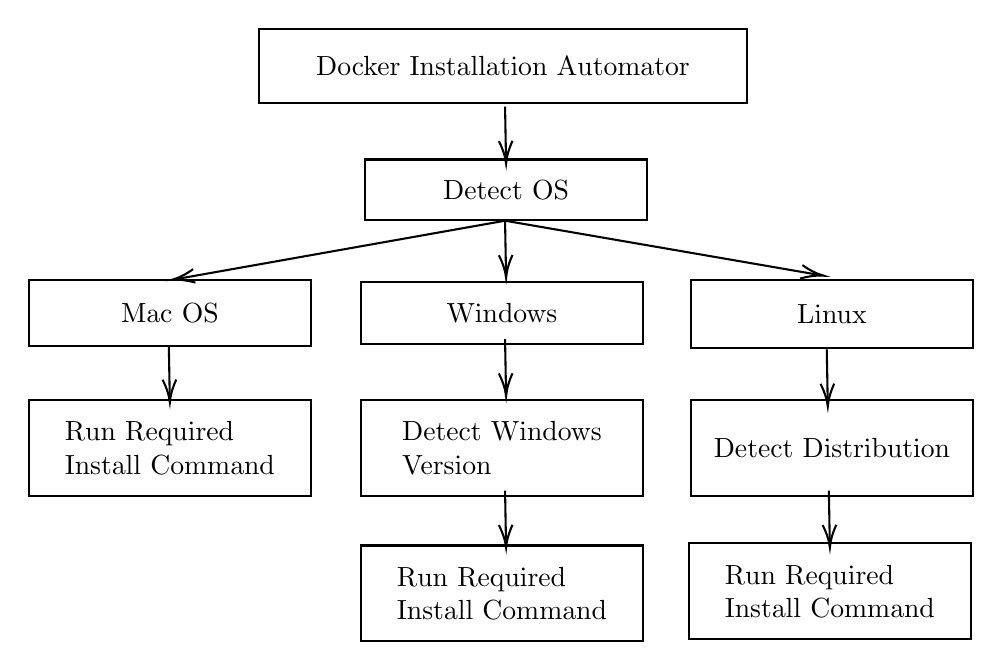
\begin{tikzpicture}[x=0.75pt,y=0.75pt,yscale=-1,xscale=1]
%uncomment if require: \path (0,387); %set diagram left start at 0, and has height of 387
%Shape: Rectangle [id:dp12391033482252478]
\draw   (232.5,102) -- (368.5,102) -- (368.5,131) -- (232.5,131) -- cycle ;
%Shape: Rectangle [id:dp2555094989002722]
\draw   (181.5,39) -- (416.5,39) -- (416.5,75) -- (181.5,75) -- cycle ;
%Shape: Rectangle [id:dp03162657543059133]
\draw   (70.5,160) -- (206.5,160) -- (206.5,192) -- (70.5,192) -- cycle ;
%Shape: Rectangle [id:dp1947521533199792]
\draw   (230.5,161) -- (366.5,161) -- (366.5,191) -- (230.5,191) -- cycle ;
%Shape: Rectangle [id:dp39981703441594085]
\draw   (389.5,160) -- (525.5,160) -- (525.5,193) -- (389.5,193) -- cycle ;
%Shape: Rectangle [id:dp5445432499512475]
\draw   (389.5,218) -- (525.5,218) -- (525.5,264) -- (389.5,264) -- cycle ;
%Shape: Rectangle [id:dp16820618798873133]
\draw   (388.5,287) -- (524.5,287) -- (524.5,333) -- (388.5,333) -- cycle ;
%Shape: Rectangle [id:dp200391241880703]
\draw   (230.5,288) -- (366.5,288) -- (366.5,334) -- (230.5,334) -- cycle ;
%Shape: Rectangle [id:dp30770436978288385]
\draw   (230.5,218) -- (366.5,218) -- (366.5,264) -- (230.5,264) -- cycle ;
%Shape: Rectangle [id:dp693797802592405]
\draw   (70.5,218) -- (206.5,218) -- (206.5,264) -- (70.5,264) -- cycle ;
%Straight Lines [id:da8290451967136283]
\draw    (300,76.5) -- (300.46,102) ;
\draw [shift={(300.5,104)}, rotate = 268.96] [color={rgb, 255:red, 0; green, 0; blue, 0 }  ][line width=0.75]    (10.93,-3.29) .. controls (6.95,-1.4) and (3.31,-0.3) .. (0,0) .. controls (3.31,0.3) and (6.95,1.4) .. (10.93,3.29)   ;
%Straight Lines [id:da46504760658282174]
\draw    (300,131.5) -- (300.46,157) ;
\draw [shift={(300.5,159)}, rotate = 268.96] [color={rgb, 255:red, 0; green, 0; blue, 0 }  ][line width=0.75]    (10.93,-3.29) .. controls (6.95,-1.4) and (3.31,-0.3) .. (0,0) .. controls (3.31,0.3) and (6.95,1.4) .. (10.93,3.29)   ;
%Straight Lines [id:da697562345132964]
\draw    (300,188.5) -- (300.46,214) ;
\draw [shift={(300.5,216)}, rotate = 268.96] [color={rgb, 255:red, 0; green, 0; blue, 0 }  ][line width=0.75]    (10.93,-3.29) .. controls (6.95,-1.4) and (3.31,-0.3) .. (0,0) .. controls (3.31,0.3) and (6.95,1.4) .. (10.93,3.29)   ;
%Straight Lines [id:da29460818271989786]
\draw    (300,261.5) -- (300.46,287) ;
\draw [shift={(300.5,289)}, rotate = 268.96] [color={rgb, 255:red, 0; green, 0; blue, 0 }  ][line width=0.75]    (10.93,-3.29) .. controls (6.95,-1.4) and (3.31,-0.3) .. (0,0) .. controls (3.31,0.3) and (6.95,1.4) .. (10.93,3.29)   ;
%Straight Lines [id:da12315236334431812]
\draw    (455,193.5) -- (455.46,219) ;
\draw [shift={(455.5,221)}, rotate = 268.96] [color={rgb, 255:red, 0; green, 0; blue, 0 }  ][line width=0.75]    (10.93,-3.29) .. controls (6.95,-1.4) and (3.31,-0.3) .. (0,0) .. controls (3.31,0.3) and (6.95,1.4) .. (10.93,3.29)   ;
%Straight Lines [id:da4360797681426818]
\draw    (138,191.5) -- (138.46,217) ;
\draw [shift={(138.5,219)}, rotate = 268.96] [color={rgb, 255:red, 0; green, 0; blue, 0 }  ][line width=0.75]    (10.93,-3.29) .. controls (6.95,-1.4) and (3.31,-0.3) .. (0,0) .. controls (3.31,0.3) and (6.95,1.4) .. (10.93,3.29)   ;
%Straight Lines [id:da47355294652329594]
\draw    (456,261.5) -- (456.46,287) ;
\draw [shift={(456.5,289)}, rotate = 268.96] [color={rgb, 255:red, 0; green, 0; blue, 0 }  ][line width=0.75]    (10.93,-3.29) .. controls (6.95,-1.4) and (3.31,-0.3) .. (0,0) .. controls (3.31,0.3) and (6.95,1.4) .. (10.93,3.29)   ;
%Straight Lines [id:da6592684678579579]
\draw    (300,131.5) -- (451.53,157.66) ;
\draw [shift={(453.5,158)}, rotate = 189.79] [color={rgb, 255:red, 0; green, 0; blue, 0 }  ][line width=0.75]    (10.93,-3.29) .. controls (6.95,-1.4) and (3.31,-0.3) .. (0,0) .. controls (3.31,0.3) and (6.95,1.4) .. (10.93,3.29)   ;
%Straight Lines [id:da5603048049658739]
\draw    (300,131.5) -- (141.47,159.65) ;
\draw [shift={(139.5,160)}, rotate = 349.93] [color={rgb, 255:red, 0; green, 0; blue, 0 }  ][line width=0.75]    (10.93,-3.29) .. controls (6.95,-1.4) and (3.31,-0.3) .. (0,0) .. controls (3.31,0.3) and (6.95,1.4) .. (10.93,3.29)   ;
% Text Node
\draw (299,57) node  [align=left] {Docker Installation Automator};
% Text Node
\draw (300.5,116.5) node  [align=left] {Detect OS};
% Text Node
\draw (138.5,176) node  [align=left] {Mac OS};
% Text Node
\draw (298.5,176) node  [align=left] {Windows};
% Text Node
\draw (457.5,176.5) node  [align=left] {Linux};
% Text Node
\draw (457.5,241) node  [align=left] {Detect Distribution};
% Text Node
\draw (456.5,310) node  [align=left] {Run Required\\Install Command};
% Text Node
\draw (298.5,311) node  [align=left] {Run Required\\Install Command};
% Text Node
\draw (298.5,241) node  [align=left] {Detect Windows\\Version};
% Text Node
\draw (138.5,241) node  [align=left] {Run Required\\Install Command};
\end{tikzpicture}

  \caption{Automated Docker Installation Process}
  \label{fig:install}
\end{figure}

\begin{algorithm}[H]
  \SetKwInOut{Input}{input}
\SetKwInOut{Output}{output}
\SetKwProg{Fn}{Function}{}{end}
\Fn{install()}{
  \Output{A message of if Docker is properly installed}
  $OS\leftarrow$platform.system() \\
  \uIf{OS == Linux}{
    $distro\leftarrow$platform.linux\_distribution()
  }
  \uElseIf{OS == Mac OS}{
    $distro\leftarrow$MacOS
  }
  \uElseIf{OS == Windows}{
    $distro\leftarrow$Windows
  }
  $file\leftarrow$get\_instructions($distro$)\\
  execute\_instructions($file$)
}
\SetKwProg{Fn}{Function}{}{end}
\Fn{get\_instructions($distro$)}{
  \Input{$distro\leftarrow$ The name of the instruction set to load}
  \Output{$file\leftarrow$ Filepath to the corresponding instruction set for $distro$}
  \If{$distro$ == distro\_name}{
    $file\leftarrow$ $file\_path$
  }
  return $file$
}
\SetKwProg{Fn}{Function}{}{end}
\Fn{execute\_instructions($file$)}{
  \Input{$file$: The path to the instruction set for the host machine}
  \Output{True or False, corresponding to if there are any issues faced during command execution}
  $commands\leftarrow$open($file$, \'r\')
  \For{$command$ in $commands$}{
    os.system($command$)
    \If{Issue faced}{
      return $False$
    }
  }
  return $True$
}
\Fn{confirm\_installation()}{
  $installed\leftarrow$ $False$ \\
  docker run $hello-world$ \\
  \If{No Issues}{
    $installed\leftarrow$ $True$
  }
  return $installed$
}

  \caption{Installation Algorithm Pseudo Code}
  \label{alg:install}
\end{algorithm}


\section{Interface}
\label{sec:interface}

The goal of the interface is to streamline the user experience interacting with the more common Docker elements like running and deleting both Docker containers and Docker images. Another goal is to have the interface be visually appealing to allow for extended use of the interface.

The Interface itself utilizes a combination of HTML, CSS, JavaScript, and the Python Flask \cite{flask} framework to create the interface as a webpage that can be viewed in any web browser. This switch from utilizing a direct GUI package as described in the Proposal is due in part to the goal of ensuring that this system will be able to work with nearly every operating system. An additional reason for the switch between a dedicated GUI and Flask is the ease of developing the interface itself. With many of the GUI packages, I researched the level of customization and design was not very high, added to this was the level of difficulty that I would have faced trying to get every element to work properly and be located within the correct area.

The Interface is broken up into several different pages for the different types of functions. The first page is for functions dedicated to the creation, management, and running of Docker images. This includes a function to generate a Dockerfile for a given directory utilizing the Dockerfile Generator tool included. The next page is for functions dedicated to the creation, management, and running of Docker containers. For each page, the different functions utilize forms to submit any required information to the Flask endpoints utilizing Post methods. There is also a button on the sidebar which allows the user to shut down the tool from the interface. Images of the two main pages of the Interface, one for Images and the other for Containers can be seen below in image \ref{img:ImagesPage}.

\begin{figure}[h!]
  \centering
  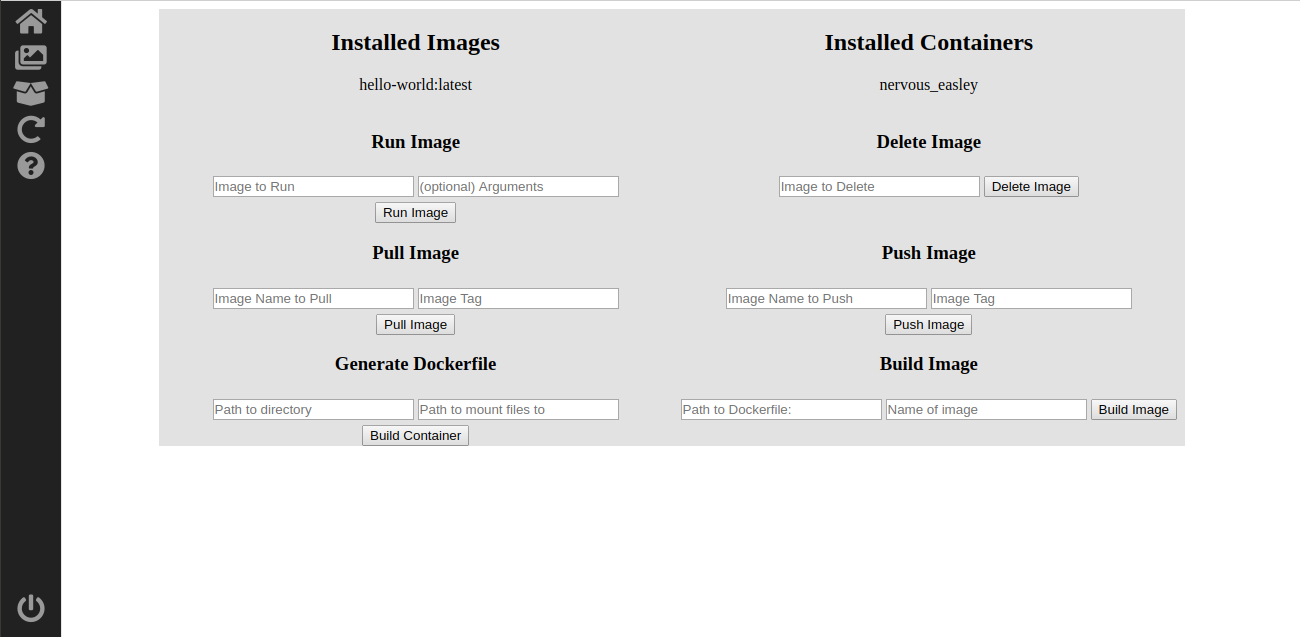
\includegraphics[width=5in]{images/InterfaceImages}
  \caption{Interface Images Page}
  \label{img:ImagesPage}
\end{figure}

Other than the visual interface there is also a command-line that can be used to interact with Docker. This aspect was included for cases where a browser-based interface may not be practical or necessary. It was also created to test functions as they were developed and instead of removing it was integrated into the overall tool. The command line has all of the same functions as the interface and can be more responsive due to not having to wait for a page to finish loading in the browser.


\section{Generator}
\label{sec:generator}

The Dockerfile Generator relies on several assumptions to work properly. These assumptions do not necessarily hurt the user's experience though with more advanced users of Linux could, in theory, have some sort of effect. The first assumption that the generator makes is that after being pointed to a directory on the host machine that the user would like to make it so that every program file within the directory is runnable. This assumption is made to decrease the number of choices that the user has to make and in doing so has a higher degree of automation for the process. Another assumption made in this regard is that if a user has multiple types of programs in the same file, they will at some point want to run each of those program files.

The next assumption that the Generator makes is that the user will not care what distribution of Linux the image is built on top of. The image the Dockerfile and the subsequent image is based on is Debian:Bullseye, which like Ubuntu, the Linux distro that I am most familiar with, uses the Apt package manager. This assumption is currently hardcoded into the Dockerfile Generator, though in the future it could be possible to modify the Generator to allow further customization of which distribution the image is based on.

The hard coding of the distribution used for the Generator is what ensures that the generator knows what package to download and install for each language. This is necessary due to there not being a default naming scheme across package managers, nor a centralized list of available packages for every programming language and package manager. As of February 28th, the Generator supports the installation of several programming languages. This list consists of Python, Java, Ruby, C, C\#, Go, JavaScript (Node.js), though adding new languages is easy to do.

\begin{figure}[h!]
  \centering
  


\tikzset{every picture/.style={line width=0.75pt}} %set default line width to 0.75pt

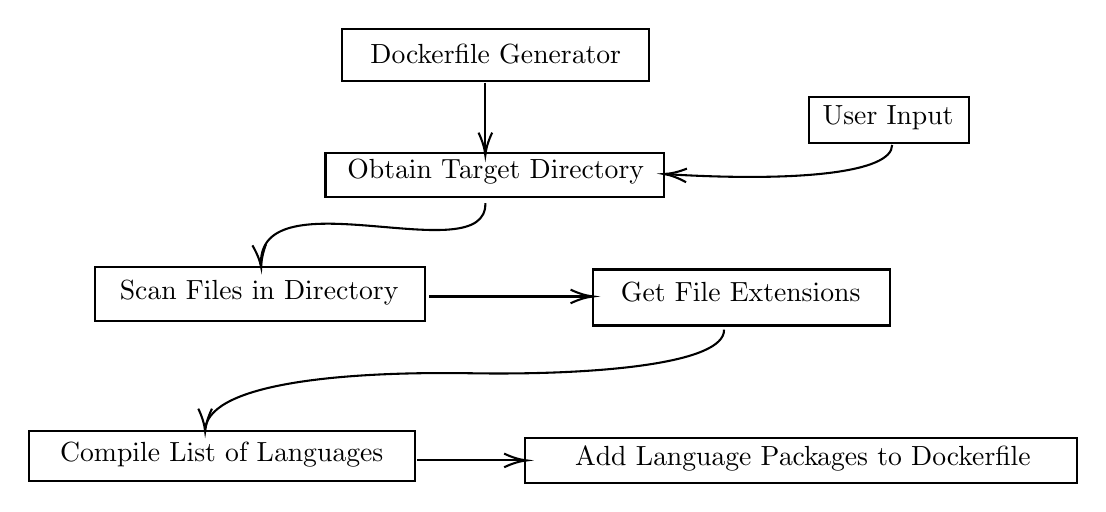
\begin{tikzpicture}[x=0.75pt,y=0.75pt,yscale=-1,xscale=1]
%uncomment if require: \path (0,447); %set diagram left start at 0, and has height of 447

%Shape: Rectangle [id:dp6708330246204339]
\draw   (254,19) -- (402,19) -- (402,44) -- (254,44) -- cycle ;
%Shape: Rectangle [id:dp3690663496827087]
\draw   (246,79) -- (409,79) -- (409,100) -- (246,100) -- cycle ;
%Shape: Rectangle [id:dp04032174080708906]
\draw   (479,52) -- (556,52) -- (556,74) -- (479,74) -- cycle ;
%Shape: Rectangle [id:dp3663336326705653]
\draw   (135,134) -- (294,134) -- (294,160) -- (135,160) -- cycle ;
%Shape: Rectangle [id:dp1296990044512687]
\draw   (375,135) -- (518,135) -- (518,162) -- (375,162) -- cycle ;
%Shape: Rectangle [id:dp5900699675454877]
\draw   (103,213) -- (289,213) -- (289,237) -- (103,237) -- cycle ;
%Shape: Rectangle [id:dp5669318997590742]
\draw   (342,216) -- (608,216) -- (608,238) -- (342,238) -- cycle ;
%Straight Lines [id:da9499154626346906]
\draw    (323,45) -- (323,78) ;
\draw [shift={(323,80)}, rotate = 270] [color={rgb, 255:red, 0; green, 0; blue, 0 }  ][line width=0.75]    (10.93,-3.29) .. controls (6.95,-1.4) and (3.31,-0.3) .. (0,0) .. controls (3.31,0.3) and (6.95,1.4) .. (10.93,3.29)   ;
%Curve Lines [id:da07473585010478478]
\draw    (519,75) .. controls (519,88.37) and (473.92,92.91) .. (410.91,89.12) ;
\draw [shift={(409,89)}, rotate = 363.58000000000004] [color={rgb, 255:red, 0; green, 0; blue, 0 }  ][line width=0.75]    (10.93,-3.29) .. controls (6.95,-1.4) and (3.31,-0.3) .. (0,0) .. controls (3.31,0.3) and (6.95,1.4) .. (10.93,3.29)   ;
%Curve Lines [id:da3255234731100256]
\draw    (323,103) .. controls (323.99,136.66) and (213.25,88.97) .. (214.91,132.65) ;
\draw [shift={(215,134)}, rotate = 265.03] [color={rgb, 255:red, 0; green, 0; blue, 0 }  ][line width=0.75]    (10.93,-3.29) .. controls (6.95,-1.4) and (3.31,-0.3) .. (0,0) .. controls (3.31,0.3) and (6.95,1.4) .. (10.93,3.29)   ;
%Straight Lines [id:da9168787921818711]
\draw    (296,148) -- (373,148) ;
\draw [shift={(375,148)}, rotate = 180] [color={rgb, 255:red, 0; green, 0; blue, 0 }  ][line width=0.75]    (10.93,-3.29) .. controls (6.95,-1.4) and (3.31,-0.3) .. (0,0) .. controls (3.31,0.3) and (6.95,1.4) .. (10.93,3.29)   ;
%Curve Lines [id:da18630293162808487]
\draw    (438,164) .. controls (438.48,180.4) and (377,186) .. (316,185) .. controls (256.52,184.03) and (191.35,189.42) .. (188.12,211.29) ;
\draw [shift={(188,213)}, rotate = 270] [color={rgb, 255:red, 0; green, 0; blue, 0 }  ][line width=0.75]    (10.93,-3.29) .. controls (6.95,-1.4) and (3.31,-0.3) .. (0,0) .. controls (3.31,0.3) and (6.95,1.4) .. (10.93,3.29)   ;
%Straight Lines [id:da8834662262571595]
\draw    (290,227) -- (341,227) ;
\draw [shift={(343,227)}, rotate = 180] [color={rgb, 255:red, 0; green, 0; blue, 0 }  ][line width=0.75]    (10.93,-3.29) .. controls (6.95,-1.4) and (3.31,-0.3) .. (0,0) .. controls (3.31,0.3) and (6.95,1.4) .. (10.93,3.29)   ;

% Text Node
\draw (328,31) node   [align=left] {Dockerfile Generator};
% Text Node
\draw (328,88) node   [align=left] {Obtain Target Directory};
% Text Node
\draw (517,62) node   [align=left] {User Input};
% Text Node
\draw (214,146) node   [align=left] {Scan Files in Directory};
% Text Node
\draw (446,146) node   [align=left] {Get File Extensions};
% Text Node
\draw (196,224) node   [align=left] {Compile List of Languages};
% Text Node
\draw (476,226) node   [align=left] {Add Language Packages to Dockerfile};


\end{tikzpicture}

  \caption{Dockerfile Generation Process}
  \label{fig:generator}
\end{figure}

\begin{algorithm}[H]
  \SetKwInOut{Input}{input}
\SetKwInOut{Output}{output}
\SetKwProg{Fn}{Function}{}{end}
\Fn{generate\_dockerfile($directory$, $to\_dir$ \= "project/")}{
  \Input{The directory to generate the Dockerfile for and optionally where to place the files to be run in the container}
  \Output{A Dockerfile which installs all required languages}

  $FILE\_TYPES\leftarrow$Dictionary of langauge packages and language extensions

  $extensions\leftarrow$get\_file\_types($directory$) \\
  \For{$ext$ in $extensions$}{
    $installs$ += FILE\_TYPES[$ext$]
  }
  Write Dockerfile with included $installs$
}

\SetKwProg{Fn}{Function}{}{end}
\Fn{get\_file\_types($directory$)}{
  \Input{The directory to analyze for file types}
  \Output{A Set of filetypes extensions found in $directory$}
  $filetypes\leftarrow$Set\\
  \For{file in $directory$}{
    $filetypes\leftarrow$file extension
  }
return $filetypes$
}

  \caption{Generator Algorithm Pseudocode}
  \label{alg:generate}
\end{algorithm}

The Generator itself works by scanning the inputted directory for files. Each file is then checked for a filetype. This is where the third main assumption is made, the Generator currently assumes that every program file utilizes a standard file extension to denote its language. In other words, Python files end with .py (and are written in Python3, though due to an upcoming depreciation of Python2 is not an invalid assumption) and Java files end with .java. This assumption is not necessarily bad, though having methods that analyze the contents of the file, especially in the case of there not being a file extension, would be greatly beneficial to the Generator.

As each file is checked the file extension is added to a set which ensures that there are no duplicate installs written into the Dockerfile. Once all files within the directory have been analyzed, the resulting filetypes set is then compared against a dictionary of known packages and each language that is found is written into the Dockerfile to be installed on the image. This overall process is illustrated in figure \ref{fig:generator} and the pseudocode for this process can be seen in Algorithm \ref{alg:generate} and a more detailed explanation of the process can be read in the following paragraph.

To identify programming languages used within a folder, I utilized the built-in OS package of Python, specifically the walk() method. This method is then supplied the path to the folder from the Home directory and returns a tuple containing the directory path, directory names, and files names within that folder. This information is reduced down to just the file names as the directory path and names are not pertinent to this operation. To ensure that the files being checked are only program files the names are passed through a regex (r'\textasciicircum[a-zA-Z0-9\_]+\textbackslash.[a-zA-Z0-9\_]+\$'). This process allows for letters and numbers as well as other special characters, but requires that there is a file type extension that can be extracted. The file types are then collected by splitting the file names and adding the resulting extension to a Set. Finally, the set is compared to a known list of file type extensions stored within a dictionary to determine the required packages for installation.

The information given above in section \ref{sec:tools} through section \ref{sec:generator} provide a look into the lower level of how the tool works to accomplish the goal presented in the Thesis Outline \ref{sec:outline}. How well the tool accomplishes this will be discussed within the Experimental Results section \ref{ch:experiments}.
